\documentclass[12pt,a4paper]{report}

\usepackage{geometry}
\usepackage{graphicx}
\usepackage{longtable}
\usepackage{pgfgantt}
\usepackage[dutch]{babel}
\usepackage{url}
\usepackage{pgf,pgfplots}
\usetikzlibrary{fit,calc}
\usepgfplotslibrary{external}

\geometry{a4paper}

\newcommand{\boxplot}[6]{%
	%#1: center, #2: median, #3: 1/4 quartile, #4: 3/4 quartile, #5: min, #6: max
	\filldraw[fill=white,line width=0.2mm] let \n{boxxl}={#1-0.1}, \n{boxxr}={#1+0.1} in (axis cs:\n{boxxl},#3) rectangle (axis cs:\n{boxxr},#4);   % draw the box
	\draw[line width=0.2mm, color=red] let \n{boxxl}={#1-0.1}, \n{boxxr}={#1+0.1} in (axis cs:\n{boxxl},#2) -- (axis cs:\n{boxxr},#2);             	% median
	\draw[line width=0.2mm] (axis cs:#1,#4) -- (axis cs:#1,#6);                                                                           							% bar up
	\draw[line width=0.2mm] let \n{whiskerl}={#1-0.025}, \n{whiskerr}={#1+0.025} in (axis cs:\n{whiskerl},#6) -- (axis cs:\n{whiskerr},#6);        % upper quartile
	\draw[line width=0.2mm] (axis cs:#1,#3) -- (axis cs:#1,#5);                                                                           							% bar down
	\draw[line width=0.2mm] let \n{whiskerl}={#1-0.025}, \n{whiskerr}={#1+0.025} in (axis cs:\n{whiskerl},#5) -- (axis cs:\n{whiskerr},#5);        % lower quartile
}

\title{P\&O Computerwetenschappen - Verslag}
\author{Team Platinum}

\begin{document}

\maketitle
\tableofcontents

\begin{abstract}
Tijdens de uitwerking van dit jaar-overschrijdend groepswerk, bouwen wij een autonome robot met behulp van Lego Mindstorms. Voor de programmatie wordt beroep gedaan op Lejos, een Open Bron project dat een minimale JAVA virtuele machine heeft gemaakt die de plaats kan innemen van de standaard programmatie omgeving van Lego.

Naast de doelstelling om kennis te maken met het ontwikkelen van een autonome robot, willen we in dit project ook ervaring opdoen ivm het werken in team verband aan een middelgroot softwareproject. Hierbij zijn organisatie van werk, planning, analyse, architectuur,... belangrijke begrippen.

Parallel met het verplicht te volgen traject van meerdere demo sessies, kiezen we voor een traject waarbij het uiteindelijke doel van het project voorop wordt gesteld: een volledig onbekend traject autonoom afleggen. Hiertoe hebben we na een korte analyse interfaces afgesproken, waar beide trajecten zich aan houden, om een vlotte integratie mogelijk te maken.

In het parallelle traject ontwikkelen we een simulator omgeving. Aan de hand van deze omgeving zijn we in staat om met meerdere teamleden in parallel een robot te ontwikkelen zonder nood aan een fysieke. Een tweede voordeel ligt in de snelheid waarmee een virtuele robot zich op een virtueel parcours kan bewegen, wat wachten tot een minimum beperkt. Tot slot is de flexibiliteit om met de debugger van een IDE door de logica van de robot te kunnen stappen van onschatbare waarde.
\end{abstract}

\chapter{Inleiding}

De tussentijdse demos helpen om de technologie stapsgewijs te verkennen. Geen van deze tussenstappen is echter rechtstreeks inzetbaar bij het effectieve doel: het autonoom rijden van een onbekend traject.

We kiezen er voor om ons team op te splitsen en twee verschillende trajecten te volgen: \'e\'en dat zich toelegt op het optimaal implementeren van de tussentijdse opdrachten en \'e\'en dat er voor zorgt dat een volledige architectuur uitgewerkt wordt die ons zal toelaten om de eindopdracht optimaal te realiseren.

Op basis van een architectuur studie werden de componenten van de eindoplossing ge\"identificeerd. In een Work Breakdown Structure\footnote{\url{http://en.wikipedia.org/wiki/Work_breakdown_structure}} (WBS) werden vervolgens de deelstappen opgelijst, toegewezen aan verantwoordelijken en deadlines bepaald. Deze informatie vormde de basis voor een planning. De WBS en planning zijn opgenomen in respectievelijk bijlagen \ref{appendix:wbs} en \ref{appendix:planning}

\section{Architectuur}

De architectuur die we zullen implementeren in dit project richt zich op het realiseren van een robuuste oplossing; zowel op het vlak van de autonome robot als ook op het volledige framework er rond dat we opbouwen op de PC. Figuur \ref{fig:architectuur} geeft de algemene architectuur weer. We belichten vervolgens de architectuur vanuit het oogpunt van beide omgevingen waar de oplossing zal actief zijn: de robot en de PC.

\begin{figure}[htbp]
   \centering
   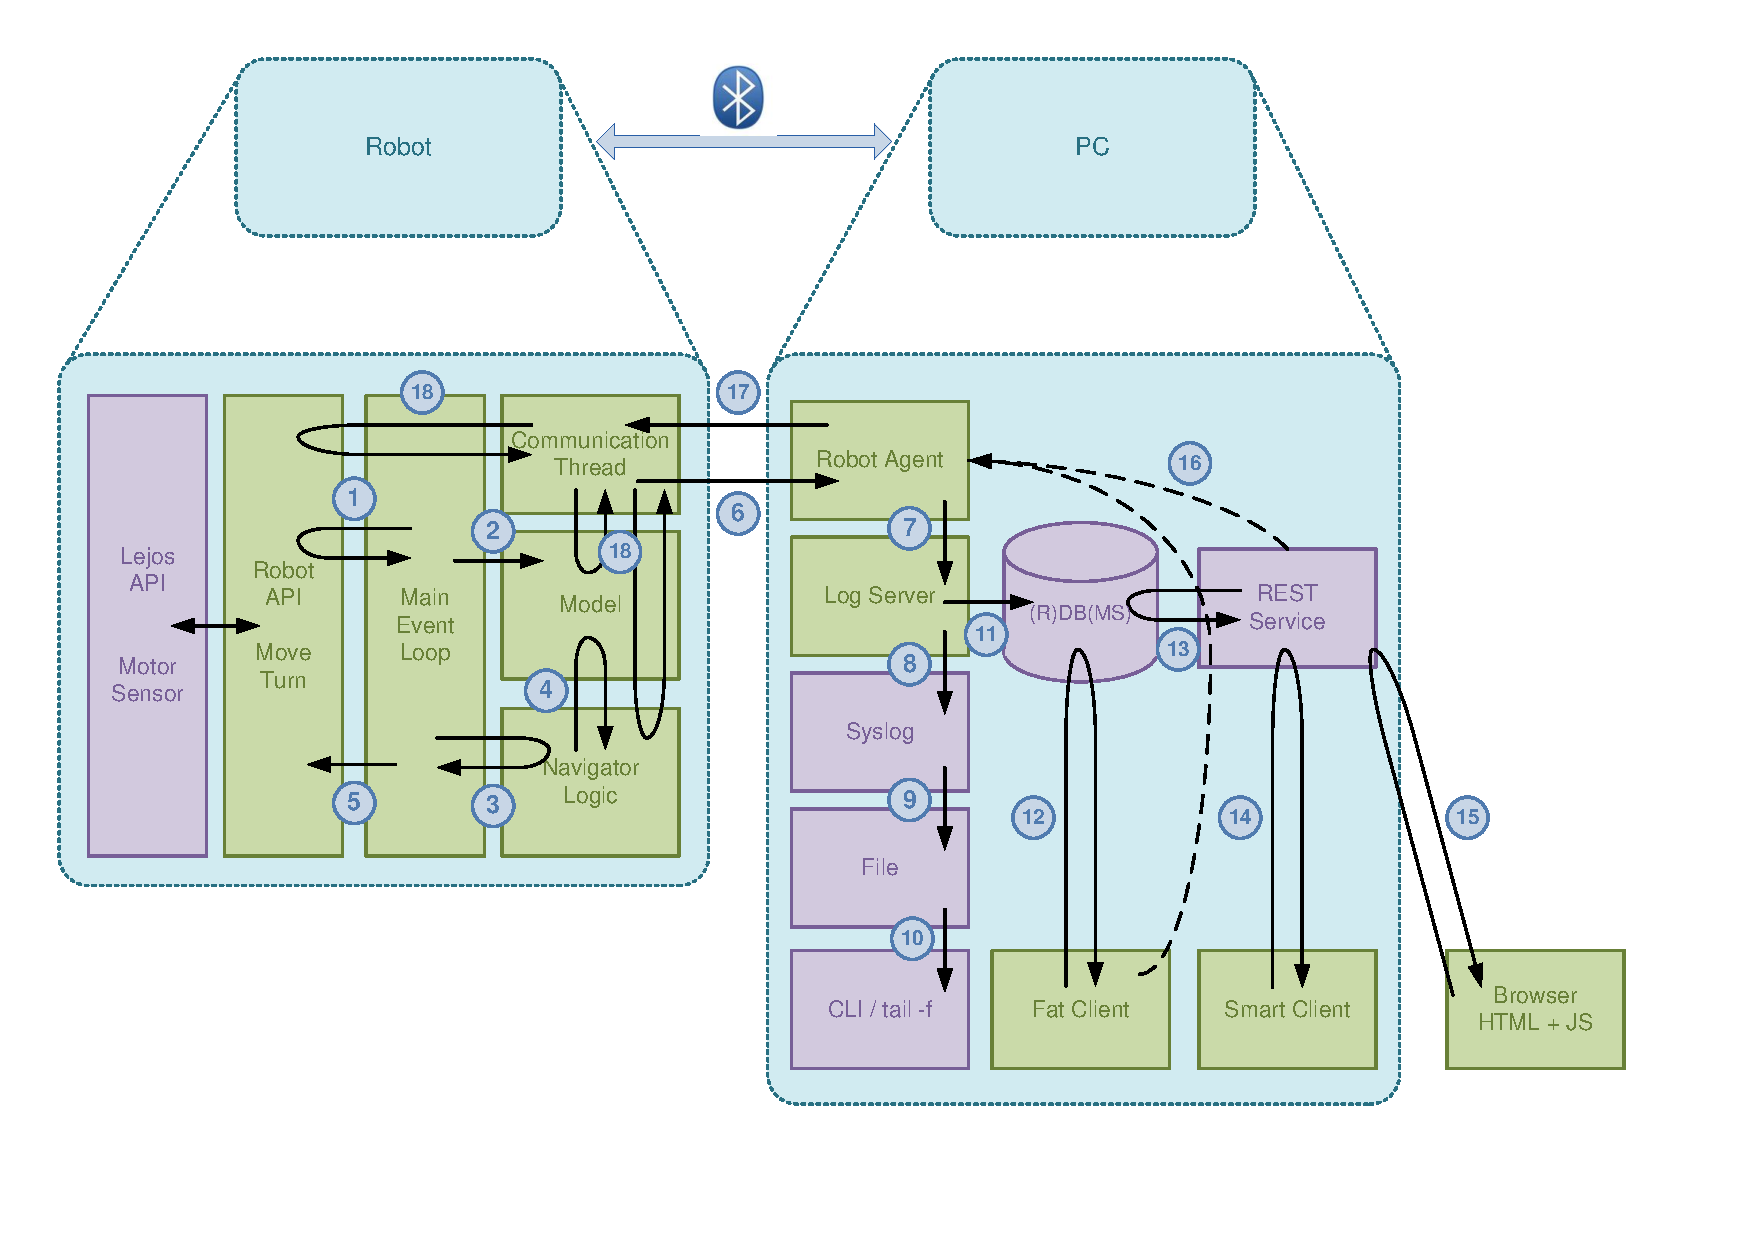
\includegraphics[width=200mm, angle=90]{resources/architectuur.pdf}
   \caption{Architectuur}
   \label{fig:architectuur}
\end{figure}

\subsection{Robot}

De robot biedt een technische API die toegang verleent tot de motoren en sensoren. We kiezen er voor om een eigen RobotAPI te introduceren die abstractie maakt van de technische API. Deze zal ons toelaten een andere implementatie te maken, die binnen een gesimuleerde omgeving gebruikt kan worden. Met deze omgeving kunnen we de logica van de robot ontwikkelen, zonder een fysieke robot.

Een tweede belangrijke component binnen de robot, wordt de �Main Event Loop�\footnote{\url{http://en.wikipedia.org/wiki/Event_loop}}. We hergebruiken hier een term die uit de wereld van de grafische gebruikers interfaces komt, maar zeer goed weergeeft wat hier gebeurt. De Main Event Loop doorloopt eindeloos 5 stappen: 

\begin{enumerate}
\item haal gegevens op van alle sensoren
\item voed de gegevens in het model
\item ondervraag de navigator welke acties dienen ondernomen te worden
\item de navigator consulteert het model om de volgende acties te bepalen
\item voer de acties uit door middel van de robot API
\end{enumerate}

Het model is een interne voorstellingsvorm van de wereld waarin de robot zich bevindt. Aan het begin van de Event Loop, zal dit model leeg zijn, of eerder volledig onbekend. Gaandeweg zal op basis van de input van de sensoren dit model gevoed worden en zal een wereldbeeld ontstaan met verschillende graden van zekerheid.

De navigator consulteert vervolgens dit model om de volgende actie te bepalen en implementeert op deze manier het ``doel'' van de robot. Deze acties worden uitgedrukt in de taal van de RobotAPI en bestaan uit functionele opdrachten zoals beweeg $x$ meter vooruit of draai $x$ graden. 

Naast de Main Event Loop, voorzien we een tweede onafhankelijke Event Loop, namelijk voor de communicatie met de PC. Deze geschiedt via Bluetooth. De redenen om deze gescheiden te houden zijn triviaal: enerzijds willen we de werking van de robot zelf niet onnodig in gevaar brengen met een proces dat kan falen. Anderzijds zal ook de frequentie waarop beide processen opereren niet gelijk lopen.

Een voorbeeld hiervan is de stroom van informatie die de lichtsensoren of sonar zullen aanbieden. Het volledig overzenden van deze gegevens kan eventueel niet mogelijk (te veel voor de beschikbare bandbreedte) of niet wenselijk (onnuttige informatie) zijn.

\subsection{PC}

Op de PC wordt alle communicatie met de robot verzorgd langs een zgn. Robot Agent. Deze extra laag zal de robuustheid van de oplossing verhogen, door het beperken van synchroon uitgevoerde code. We denken hierbij aan het rechtstreeks koppelen van de communicatie aan een gebruikersinterface.

We zijn van mening dat het louter verzenden en visualiseren van informatie over de werking van de robot een verlies aan mogelijkheden zou betekenen. Onze strategie, met een simulatieomgeving, toont al snel aan dat deze informatie kan helpen bij het onderzoek naar optimale navigator-logica.

Aangezien we de informatie dus wensen te bewaren, willen we dit ook een centraal gegeven van onze architectuur maken. Opnieuw komt dit de robuustheid van de gehele oplossing ten goede. De focus zal komen te liggen op het optimaal opslaan van de gegevens. Het visualiseren ervan komt vervolgens neer op het opvragen ervan, wat opnieuw een asynchroon proces is.

Deze architectuur heeft enkele bijkomende gevolgen. Zo wordt het bvb. mogelijk om gegevens van meerdere sessies simultaan te bekijken of kan met meerdere en/of verschillende gebruikersinterfaces gewerkt worden. Ook kan voor de realisatie van deze architectuur beroep gedaan worden op enkele standaarden, waardoor het cre\"eren van nieuwe code tot een minimum beperkt wordt.

Zo kan de Log Server ge\"implementeerd worden op basis van log4j\footnote{\url{http://logging.apache.org/log4j/}} en kan de aflevering van de inkomende communicatie volledig in configuratie gerealiseerd worden. De meest eenvoudige uitwerking kan bestaan uit het gebruiken van een syslog daemon, maar ook een relationele databank is triviaal.

Verschillende types clients kunnen de gegevens uit de databank visualiseren: een Fat Client\footnote{\url{http://en.wikipedia.org/wiki/Fat_client}} ligt voor de hand, maar ook een web-applicatie of REST\footnote{\url{http://en.wikipedia.org/wiki/Representational_state_transfer}} service zijn goede opties.

Deze laatste kan dan opnieuw gerealiseerd worden gebruikmakend van standaard componenten zoals de JBoss applicatie server\footnote{\url{http://www.jboss.org/jbossas}} en RESTeasy\footnote{\url{http://www.jboss.org/resteasy}}. Door middel van JSONP\footnote{\url{http://en.wikipedia.org/wiki/JSONP}} kan zelfs een streaming oplossing aan web-clients aangeboden worden.

\subsection{Interactie}

De architectuur (figuur \ref{fig:architectuur}) voorziet eveneens de mogelijkheid om commando's te sturen naar de robot. Aan de robot-kant zullen de meeste van de componenten handelingen registreren bij de communicatie component. Op deze manier kunnen de commando's door de communicatie component uitgevoerd worden op de geregistreerde handelingen op de componenten. Dit stelt ons in staat om op generieke manier interactief de software van de robot te ondervragen, zonder specifieke code te moeten voorzien.

\section{Functionele Analyse}

In de functionele analyse bepalen we in hoofdzaak de interfaces die gerespecteerd dienen te worden in de twee trajecten. Op basis van deze afspraken kunnen beide trajecten integreren en in elkaar opgaan.

Twee interfaces worden voorzien: de Robot interface en de RobotAPI interface. De eerste bepaalt hoe de robot opgebouwd en aangesproken kan worden door zijn omgeving. Dit kan een programma zijn dat op de robot uitgevoerd wordt, of dit kan een simulatieomgeving zijn. Ook op niveau van de RobotAPI moet deze mogelijkheid beschikbaar zijn.

\begin{figure}[htbp]
   \centering
   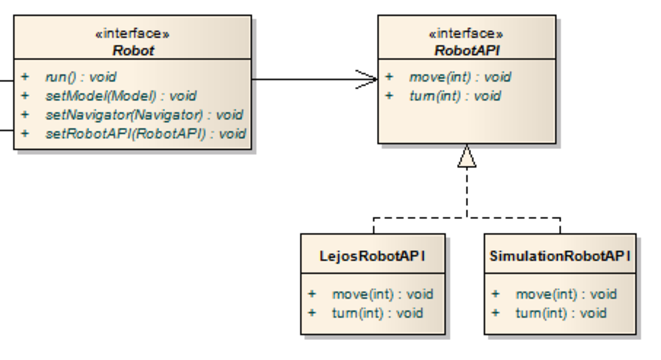
\includegraphics[width=100mm]{resources/robotapi.pdf}
    \caption{Robot \& RobotAPI}
   \label{fig:robotapi}
\end{figure}

De volledige klasse diagrammen zijn consulteerbaar in bijlage \ref{appendix:classdiagrams}.

\chapter{Demo 1: Veelhoek}

De doelstelling van de eerste demo is het rijden van een veelhoek op basis van het aantal hoeken en de lengte van een zijde. Precisie door middel van compensatie van de vast te stellen afwijkingen is hier van belang.

\section{Fysiek ontwerp}

Het ontwerp van de robot voor de eerste opdracht is het basismodel van de Mindstorms kit die we ter beschikking kregen. Gegeven het korte tijdsbestek was het belangrijker om snel ervaring op te doen met de robot. Deze ervaring kan eveneens informatie verschaffen aan het lange termijn traject.
 
\section{De software}
 
De Lejos API biedt twee mogelijkheden om de motoren aan te sturen: op basis van tijd en op basis van de omwentelingen van de wielen. Intu\"itief waren we overtuigd dat de methode op basis van omwentelingen de meest betrouwbare moest zijn.

Wat betreft de rij-technische mogelijkheden, kiezen we voor twee onafhankelijke bewegingen: het rechtdoor rijden (vooruit of achteruit) en het ter plekke draaien. Dit is enerzijds een noodzaak voor de opdracht, maar is tevens de eenvoudigste te hanteren en betrouwbaarste methode. Het draaien tijdens het rijden gaat gepaard met noodzakelijke slip- en schuifbewegingen, wat de berekenbaarheid sterk kan be"invloeden.

In beide gevallen is er nog een parameter die bepalend kan zijn: de rotatiesnelheid. Ook deze zullen we in onze testen laten vari\"eren om een optimale verhouding te vinden.

\section{Testplan en resultaten}

\subsection{Omwentelingen}

De implementatie die omwentelingen telt is afhankelijk van de omtrek van de wielen. De theoretische omtrek van het wiel kan berekend worden op basis van de diameter (56mm) en bedraagt 175,93mm.

Naast de theoretische bepaling van de omtrek voorzien we ook software die deze omtrek bepaalt op basis van een zgn. zelf-calibratie. Hierbij laten we de robot rijden, voorzien van een frontale druksensor, tot hij een obstakel raakt. Op dit ogenblik stop de robot. Vervolgens nemen we de blokkade weg en zal de robot na enkele seconden zelf verder rijden tot het volgende obstakel. Op basis van de getelde omwentelingen en de vaste afstand tussen beide obstakels, kan de robot vervolgens zelf exact de omtrek van het wiel bepalen.

De waarde die op deze manier werd vastgesteld was 175mm. Deze werd gebruikt als initi\"ele waarde.

\subsubsection{Test 1: met een vaste snelheid verschillende afstanden rijden}

Voor deze test werd de snelheid ingesteld op 400 en werden afstanden van 20, 40, 60 en 80 cm gereden. Bij de uiteindelijke opdracht wordt er gereden op een parcours dat bestaat uit panelen van 80 bij 80 cm. De robot zal zelden grotere afstanden aan \'e\'en stuk rijden.

We lieten de robot telkens 5 maal de vooropgestelde afstand rijden en berekenden vervolgens de relatieve afwijkingen. De resultaten van deze test zijn opgenomen in figuur \ref{chart:test1}.

\begin{figure}
	\caption{Test 1 : Relatieve afwijking bij vaste snelheid}
	\label{chart:test1}
	\vspace{10pt}	
	\centering
	
	\tikzset{external/remake next}
	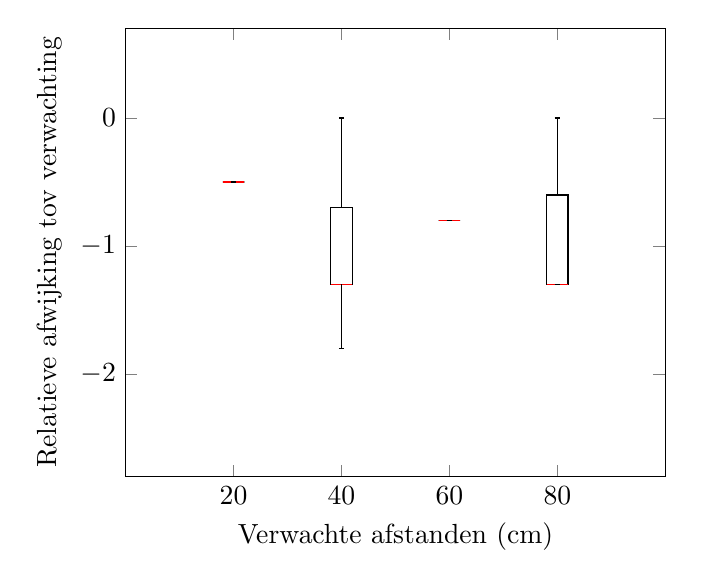
\begin{tikzpicture}
		\begin{axis}[xmin=0,xmax=5,ymin=-2.8, ymax=0.7,
			xtick={1,2,3,4,5},xticklabels={20,40,60,80},
	      		xlabel={Verwachte afstanden (cm)},
			ylabel={Relatieve afwijking tov verwachting},
			]
			%#1: center, #2: median, #3: 1/4 quartile, #4: 3/4 quartile, #5: min, #6: max
			\boxplot{1}{-0.5}{-0.5}{-0.5}{-0.5}{-0.5}
			\boxplot{2}{-1.3}{-1.3}{-0.7}{-1.8}{0}
			\boxplot{3}{-0.8}{-0.8}{-0.8}{-0.8}{-0.8}
			\boxplot{4}{-1.3}{-1.3}{-0.6}{-1.3}{0}
		\end{axis}
	\end{tikzpicture}
\end{figure}

Op basis van de resultaten, werd de wielomtrek met 1\% verkleind. Figuur \ref{chart:test1b} toont de resultaten van dezelfde test na de aanpassing.

\begin{figure}
	\caption{Test 1 : Resultaten na aanpassing wielomtrek met 1\%}
	\label{chart:test1b}
	\vspace{10pt}	
	\centering
	
	\tikzset{external/remake next}
	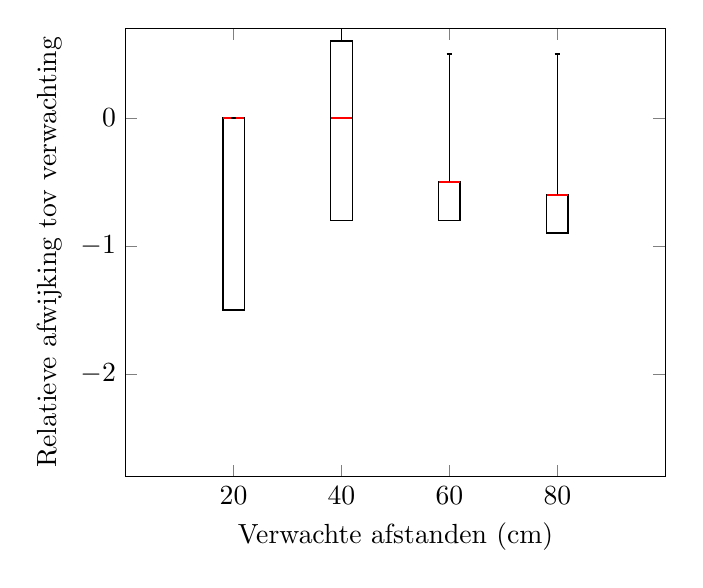
\begin{tikzpicture}
		\begin{axis}[xmin=0,xmax=5,ymin=-2.8, ymax=0.7,
			xtick={1,2,3,4,5},xticklabels={20,40,60,80},
	      		xlabel={Verwachte afstanden (cm)},
			ylabel={Relatieve afwijking tov verwachting},
			]
			%#1: center, #2: median, #3: 1/4 quartile, #4: 3/4 quartile, #5: min, #6: max
			\boxplot{1}{0}{-1.5}{0}{-1.5}{0}
			\boxplot{2}{0}{-0.8}{0.6}{-0.8}{0.8}
			\boxplot{3}{-0.5}{-0.8}{-0.5}{-0.8}{0.5}
			\boxplot{4}{-0.6}{-0.9}{-0.6}{-0.9}{0.5}
		\end{axis}
	\end{tikzpicture}
\end{figure}

\subsubsection{Test 2: een vaste afstand met verschillende snelheden}

Bij het uitvoeren van verkennende testen hadden we reeds vastgesteld dat het vertrekken, stoppen en de snelheid van de motoren een beduidende invloed hadden op de stabiliteit van de robot. Met deze tweede test willen we op zoek gaan naar een optimale snelheid/precisie verhouding.

We lieten de robot telkens 5 maal een afstand van 20cm afleggen bij vari\"erende motorsnelheden: 125, 250, 500, 750 en 1000. Vervolgens  berekenden we de relatieve afwijking. De resultaten van deze test zijn opgenomen in figuur \ref{chart:test2}.

\begin{figure}
	\caption{Test 2 : Relatieve afwijking bij variabele snelheden}
	\label{chart:test2}
	\vspace{10pt}	
	\centering
	
	\tikzset{external/remake next}
	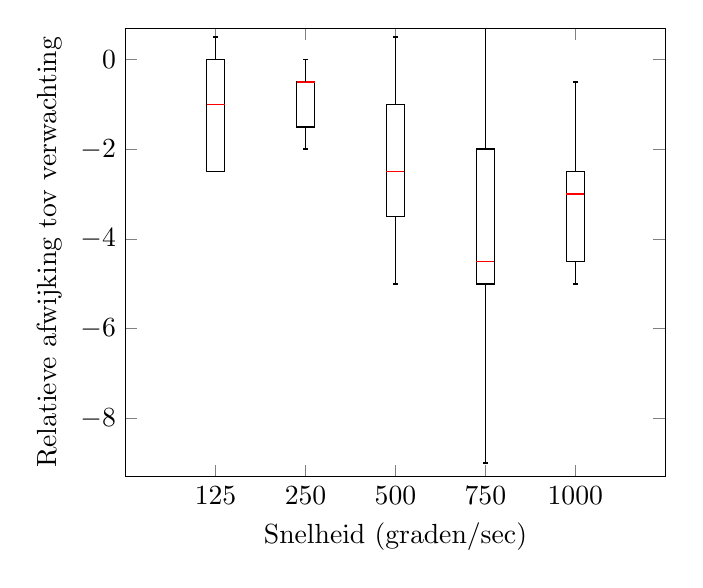
\begin{tikzpicture}
		\begin{axis}[xmin=0,xmax=6,ymin=-9.3, ymax=0.7,
			xtick={1,2,3,4,5,6},xticklabels={125,250,500,750,1000},
	      		xlabel={Snelheid (graden/sec)},
			ylabel={Relatieve afwijking tov verwachting},
			]
			%#1: center, #2: median, #3: 1/4 quartile, #4: 3/4 quartile, #5: min, #6: max
			\boxplot{1}{-1.0}{-2.5}{0}{-2.5}{0.5}
			\boxplot{2}{-0.5}{-1.5}{-0.5}{-2}{0}
			\boxplot{3}{-2.5}{-3.5}{-1.0}{-5.0}{0.5}
			\boxplot{4}{-4.5}{-5}{-2}{-9}{1.5}
			\boxplot{5}{-3.0}{-4.5}{-2.5}{-5}{-0.5}
		\end{axis}
	\end{tikzpicture}
\end{figure}

Uit de resultaten besloten we dat 250 graden per seconde ons de meest betrouwbare snelheid gaf.

Met deze snelheid werden vervolgens opnieuw verschillende afstanden gereden. De resultaten bevestigden de eerder gevonden foutmarge van ongeveer 1\%.

Dat de kwaliteit van de Lego onderdelen van groot belang kan zijn, bleek toen het omwisselen van twee wielen een oplossing bleek te zijn voor een grote afwijking naar \'e\'en bepaalde kant.

\subsubsection{Test 3: hoeken}

Het ter plekke draaien is ook gebaseerd op de wielomtrek, echter nu in combinatie met de draaicirkel die bepaald wordt door de wielafstand.

Om de nauwkeurigheid van het ter plekke draaien te bepalen, lieten we de robot 5 maal een zelfde hoek draaien. Hierbij varieerden we de hoeken als volgt: 15, 30, 45, 60 en 90 graden. Opnieuw keken we naar de eindopgave. We verwachten niet dat we met de robot veel hoeken groter dan 90 graden gaan moeten maken. Voor de veelhoek-opdracht, is dit normaal niet het geval, met een spreekwoordelijke uitzondering voor een driehoek.

Ook voor deze test wilden we de parameter snelheid in beschouwing nemen. Uit de eerste resultaten bleek snel dat een snelheid hoger dan de eerder vastgestelde 250 graden per seconde niet accepteerbare afwijkingen opleverde. Deze testen werden niet weerhouden.

De resultaten voor de verschillende hoeken zijn weergegeven in figuur \ref{chart:test3}.

\begin{figure}
	\caption{Test 3 : Relatieve afwijking bij vaste snelheid}
	\label{chart:test3}
	\vspace{10pt}	
	\centering
	
	\tikzset{external/remake next}
	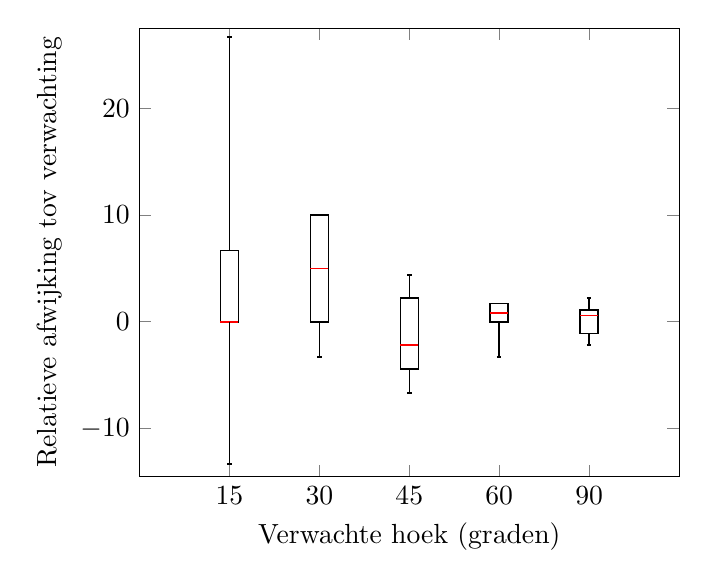
\begin{tikzpicture}
		\begin{axis}[xmin=0,xmax=6,ymin=-14.5, ymax=27.5,
			xtick={1,2,3,4,5,6},xticklabels={15,30,45,60,90},
	      		xlabel={Verwachte hoek (graden)},
			ylabel={Relatieve afwijking tov verwachting},
			]
			%#1: center, #2: median, #3: 1/4 quartile, #4: 3/4 quartile, #5: min, #6: max
			\boxplot{1}{0}{0}{6.67}{-13.3}{26.67}
			\boxplot{2}{5}{0}{10}{-3.3}{10}
			\boxplot{3}{-2.2}{-4.4}{2.2}{-6.7}{4.4}
			\boxplot{4}{0.8}{0}{1.7}{-3.3}{1.7}
			\boxplot{5}{0.6}{-1.1}{1.1}{-2.2}{2.2}
		\end{axis}
	\end{tikzpicture}
\end{figure}

De resultaten bevestigen het vermoeden dat de meetfout groter is bij kleinere hoeken. De resultaten bij 60 en 90 graden zijn dan weer positief in het kader van de einddoelstelling, waar het parcours typisch hiermee opgebouwd wordt.

\subsubsection{Conclusie ivm omwentelingen}

Met een snelheid van 250 graden per seconde en een bijstelling van de omtrek van het wiel met 1\% zou de robot, volgens onze metingen, vrij precies een willekeurige veelhoek moeten kunnen rijden.

Dit werd bevestigd bij het toepassen van deze implementatie voor het rijden van een veelhoek. Hierbij werden testen gedaan waarbij achtereenvolgens een 3, 4, 5, 6, 10 en 15-hoek werd gereden met een zijde van 20 of 30 cm. De 3, 4, 5 en 6-hoeken waren nagenoeg perfect. Bij de 10 en 15 hoek merkten we de (toen nog niet bijgewerkte) fout van 1\% op.

Figuur \ref{fig:resultsLargePolygons} toont het papier waarop we start en eindpunten aanduidden bij de grote veelhoeken en toont de afwijkingen van enkele metingen ten opzichte van het startpunt. De rode omtrek geeft de startpositie van de robot weer met het middelpunt aangegeven door het rode kruis. De zwarte kruisen zijn de middelpunten van 6 testen waarbij een 15 hoek met zijde 20 cm werd gereden.

\begin{figure}[htbp]
   \centering
   \caption{Meetresultaten voor grote veelhoeken.}
   \label{fig:resultsLargePolygons}
   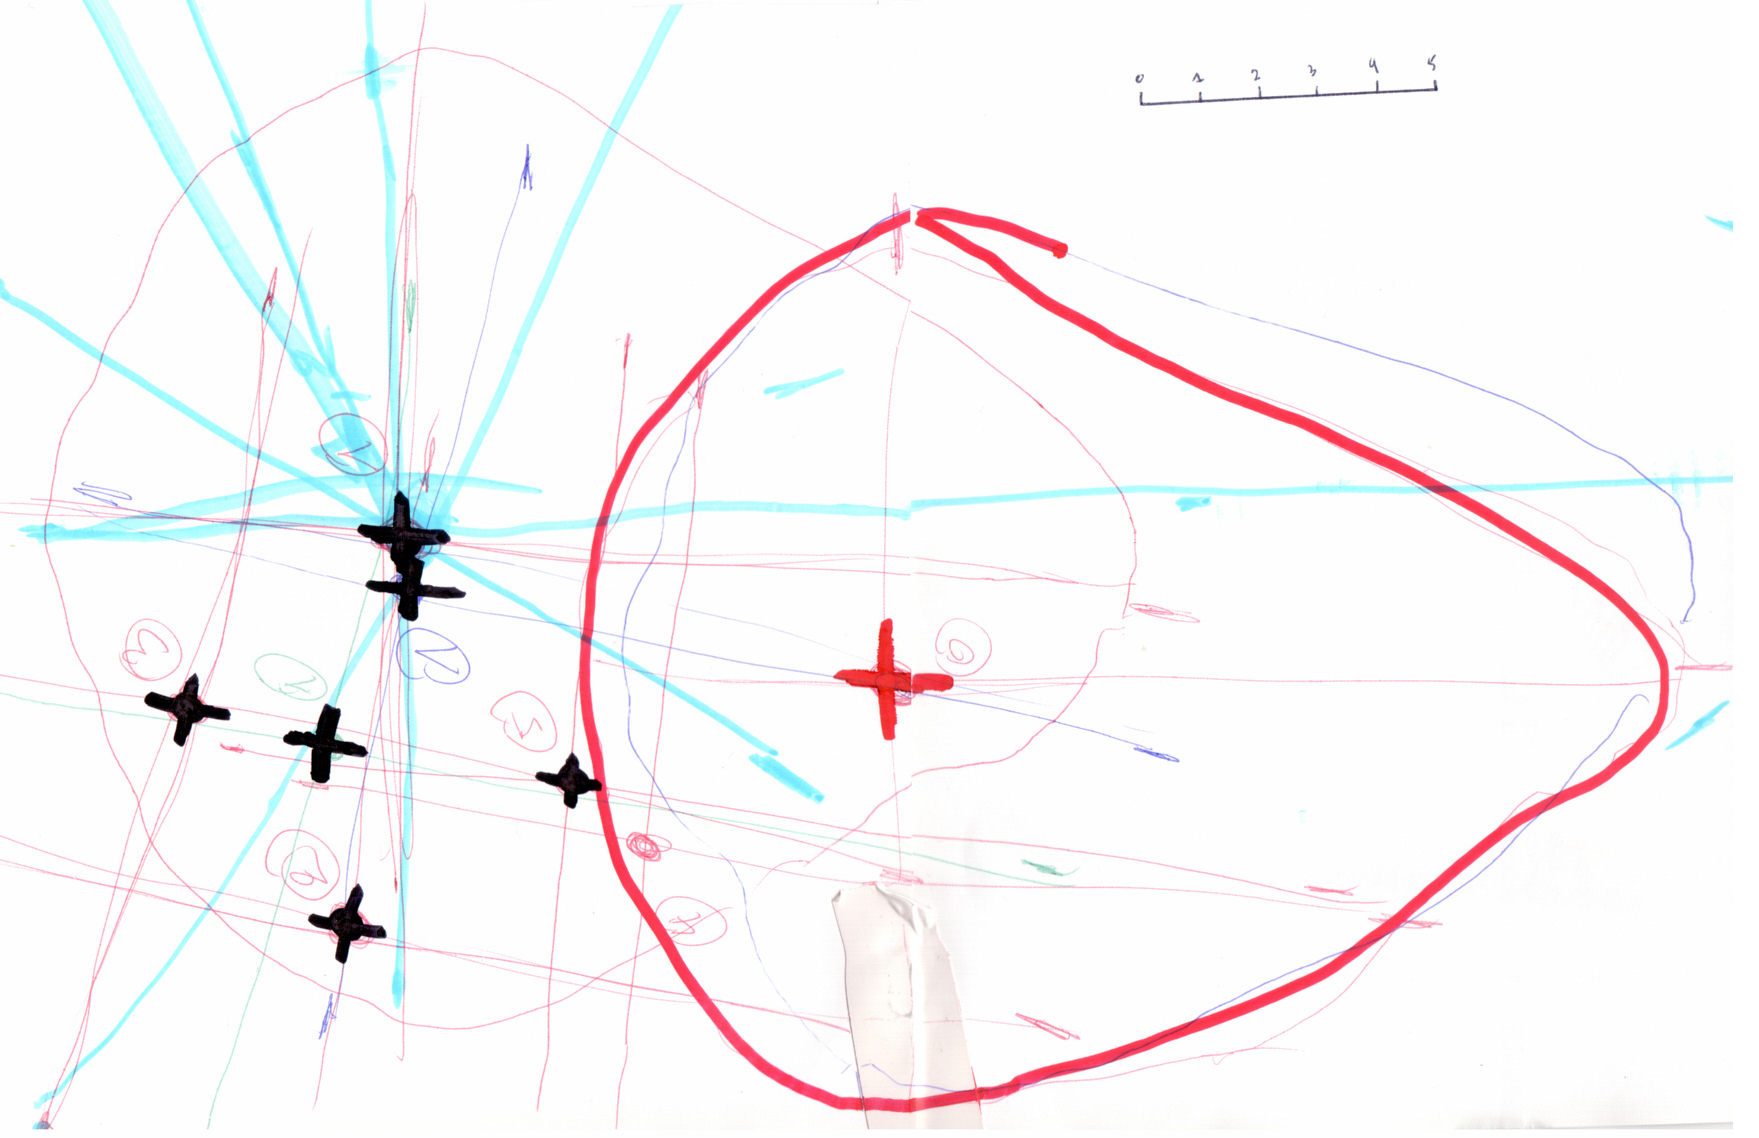
\includegraphics[width=140mm]{resources/meetresultaten.png}
\end{figure}

\subsection{Tijd}

Het aansturen van de motoren op basis van tijd bleek geen valabel alternatief te zijn. De eerste resultaten gaven procentuele afwijkingen in de grootorde van 10 tot 20\%, zodat een verdere vergelijking met de resultaten voor de omwentelingen totaal overbodig werd. Deze piste werd dan ook verlaten.

\section{Resultaten van de demo en conclusies}

Tijdens de demo werd gevraagd om een veelhoek van eigen keuze te rijden. We kozen een driehoek met een zijde van 40cm. De afwijking van het startpunt bedroeg ongeveer 10cm. De tweede veelhoek die opgegeven werd was een tienhoek met een zijde van 20cm. De afwijking van het startpunt bedroeg ongeveer 30cm.

De resultaten van de demo weken sterk af van de eerder opgetekende waarden. Uit onderzoek bleek dat het vuil worden van de wielen de oorzaak was.

Figuur \ref{chart:vervuiling} toont de evolutie van de afwijking tijdens de eerste vijf veelhoeken, gereden met init\"ieel gekuiste wielen. We merken op dat in deze grootorde van gereden veelhoeken de fout sterk stijgt. Figuur \ref{chart:vervuiling2} toont de relatieve afwijking bij 5, 10, 15, 20, 25, en 30 gereden veelhoeken.

\begin{figure}
	\caption{Relatieve afwijking tgv. vervuiling wielen}
	\label{chart:vervuiling}
	\vspace{10pt}	
	\centering
	
	\tikzset{external/remake next}
	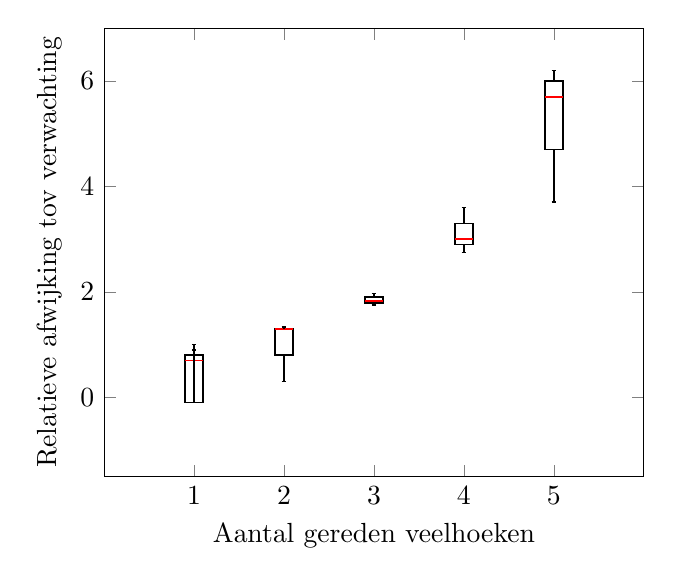
\begin{tikzpicture}
		\begin{axis}[xmin=0,xmax=6,ymin=-1.5, ymax=7,
			xtick={1,2,3,4,5,6},xticklabels={1,2,3,4,5},
	      		xlabel={Aantal gereden veelhoeken},
			ylabel={Relatieve afwijking tov verwachting},
			]
			%#1: center, #2: median, #3: 1/4 quartile, #4: 3/4 quartile, #5: min, #6: max
			\boxplot{1}{0.7}{-0.1}{0.8}{1.0}{0.9}
			\boxplot{2}{1.3}{0.8}{1.3}{0.3}{1.33}
			\boxplot{3}{1.83}{1.79}{1.9}{1.75}{1.97}
			\boxplot{4}{3.0}{2.9}{3.3}{2.75}{3.6}
			\boxplot{5}{5.7}{4.7}{6}{3.7}{6.2}
		\end{axis}
	\end{tikzpicture}
\end{figure}

\begin{figure}
	\caption{Relatieve afwijking tgv. vervuiling wielen}
	\label{chart:vervuiling2}
	\vspace{10pt}	
	\centering
	
	\tikzset{external/remake next}
	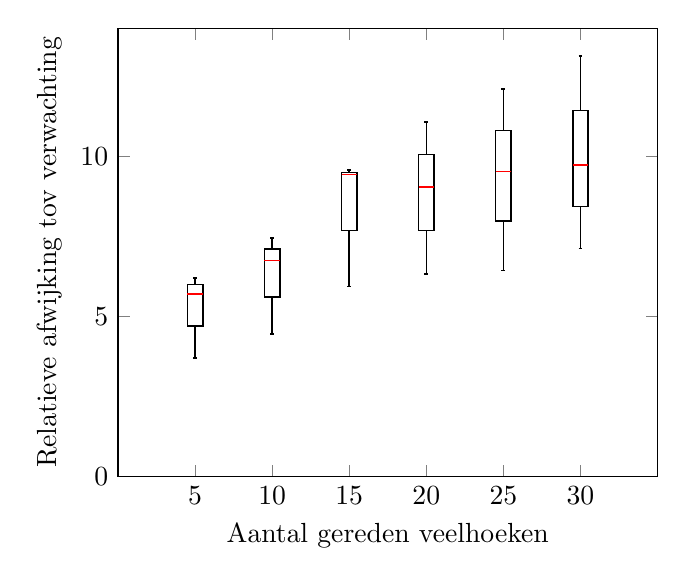
\begin{tikzpicture}
		\begin{axis}[xmin=0,xmax=7,ymin=0, ymax=14,
			xtick={1,2,3,4,5,6,7},xticklabels={5,10,15,20,25,30},
	      		xlabel={Aantal gereden veelhoeken},
			ylabel={Relatieve afwijking tov verwachting},
			]
			%#1: center, #2: median, #3: 1/4 quartile, #4: 3/4 quartile, #5: min, #6: max
			\boxplot{1}{5.7}{4.7}{6}{3.7}{6.2}
			\boxplot{2}{6.75}{5.6}{7.1}{4.45}{7.45}
			\boxplot{3}{9.43}{7.68}{9.5}{5.93}{9.57}
			\boxplot{4}{9.05}{7.69}{10.06}{6.33}{11.08}
			\boxplot{5}{9.52}{7.98}{10.81}{6.44}{12.10}
			\boxplot{6}{9.73}{8.43}{11.43}{7.12}{13.13}
		\end{axis}
	\end{tikzpicture}
\end{figure}

Uit de meting blijkt dat de fout init\"ieel sterk stijgt, maar rond 15 veelhoeken convergeert de afwijking. We zouden op basis van deze metingen kunnen besluiten dat we de robot ongeveer 15 veelhoeken zouden moeten laten rijden en vervolgens een correctie voor de gemeten fout kunnen implementeren.

Aangezien dit een specifiek probleem voor het constant rijden van veelhoeken is en dit voor de einddoelstelling geen belangrijke impact heeft, zullen we deze aanpassing niet implementeren. 

\chapter{Demo 2a: Lijnvolger}

De doelstelling van de tweede demo is het volgen van een ononderbroken lijn. Deze lijn kan wit of zwart zijn en is uitgezet op bruine panelen.

\section{Fysiek ontwerp}
\label{section:lichtsensor}

Voor het volgen van een lijn maken we gebruik van een grijswaardesensor. Deze werd vooraan op de robot bevestigd. Om de sensoren makkelijker en beter te kunnen bevestigen, werd de robot voorzien van een nieuwe structurele opbouw.

Het nieuwe design, voorgesteld in figuur \ref{fig:redesignRobot}, voorziet een opbouw waarmee een derde motor toegevoegd werd om een beweegbare sonar te realiseren. Daarnaast werden ook reeds twee druksensoren voorzien vooraan links en rechts van de robot.

\begin{figure}[htbp]
   \centering
   \caption{Redesign van het robotontwerp met alle benodigde sensoren.}
   \label{fig:redesignRobot}
   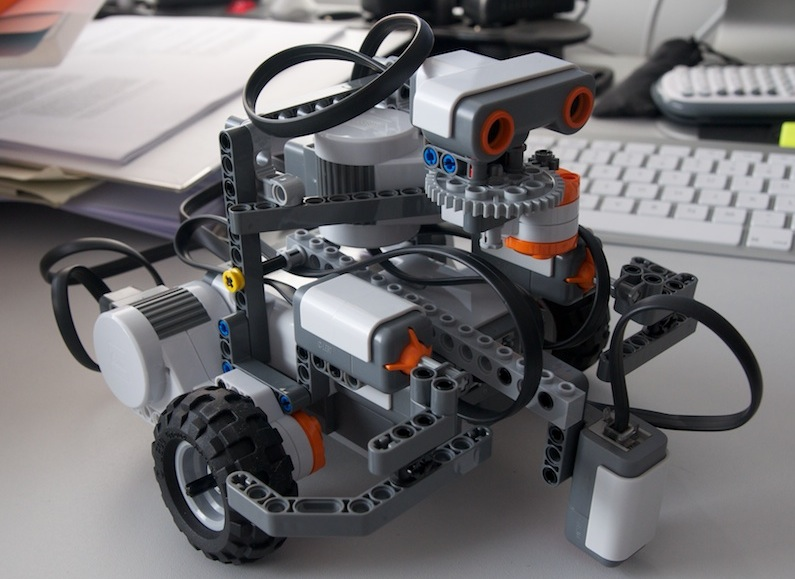
\includegraphics[width=150mm]{resources/aNGie.jpg}
\end{figure}

\section{De software}

Voor deze demo diende software ontwikkeld te worden die de robot in staat stelt om een lijn autonoom te volgen. De meetresultaten van de grijswaardesensor dienen tevens verzonden te worden via Bluetooth naar een PC, waar ze gevisualiseerd  worden. De ontwikkelingen voor robot en PC worden in dit deel verder toegelicht. De communicatie component wordt in bijlage \ref{appendix:bluetooth} in detail besproken.

\subsection{Robot}

De grijswaardesensor kan gekalibreerd worden, waarna deze genormaliseerde waarden terug geeft van 0 tot 1024\footnote{Re\"ele waarden liggen typisch tussen 145 voor een meting in een donkere omgeving en 890 in klaar zonlicht.}. Voor het kalibreren kunnen een donker- en lichtwaarde aan de Lejos API gegeven worden, welke dan gebruikt worden om de genormaliseerde waarden op af te stemmen.

Het algoritme van de robot is zeer eenvoudig gehouden, om de betrouwbaarheid te bevorderen. De volgende stappen worden in een oneindige lus uitgevoerd:

\begin{enumerate}
\item lees de genormaliseerde waarde van de grijswaardesensor
\item bepaal of de gemeten grijswaarde overeenstemt met een lijn; indien ja, rij verder rechtdoor
\item indien niet (meer) op een lijn, zoek een lijn door ter plekke heen en weer te draaien in steeds groeiende hoeken tot een lijn gevonden is
\end{enumerate}

Voor dit algoritme werd de manier waarop de Lejos API aangesproken werd gewijzigd. Voor het rijden van veelhoeken werd aan de Lejos API de opdracht gegeven om een bepaald aantal omwentelingen te doen. Vervolgens werd er gewacht om een synchrone verwerking te simuleren voor onze software. Met de introductie van sensoren en de nood om acties te ondernemen voor een bepaalde afstand bereikt is, werd deze synchrone verwerking verwijderd en zal de controle onmiddellijk teruggegeven worden aan de controleren applicatie, in dit geval het lijnvolger algoritme.

\subsection{PC}

Op de PC voorzien we een User Interface die een visuele voorstelling biedt van de door de robot opgemeten grijswaarden, gedetecteerde barcodes en bijhorende actie die ondernomen wordt. Figuur \ref{fig:demo2UI} toont de User Interface die voor de drie onderdelen van de demo zal gebruikt worden.

\begin{figure}[htbp]
   \centering
   \caption{User Interface voor Demo 2.}
   \label{fig:demo2UI}
   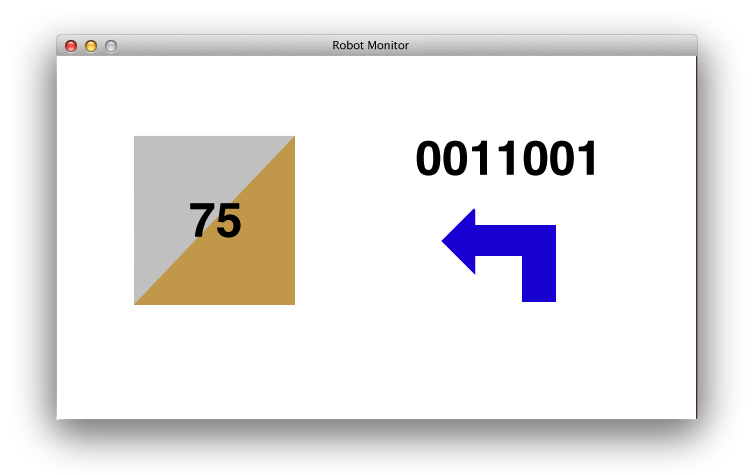
\includegraphics[width=150mm]{resources/demo2-ui.png}
\end{figure}

Aan de linkerkant wordt de gemeten grijswaarde weergegeven: als getal, als grijswaarde en als ge\"interpreteerde kleur (bruin, wit of zwart). Aan de rechterkant wordt een eventueel gedetecteerde barcode gevisualiseerd, als ook een indicatie van de actie die de robot zal uitvoeren op basis van deze informatie.

De User Interface bevat geen logica om enige conclusie te trekken en visualiseert louter de door de robot doorgestuurde gegevens. De robot stuurt dus de grijswaarde, de ge\"interpreteerde kleur, de barcode en actie door naar de PC.

\section{Testplan en resultaten}

Met de grijswaardesensor willen we drie kleuren kunnen onderscheiden: bruin, wit en zwart. De grijswaardesensor zal typisch verschillende waarden geven binnen een bepaald bereik voor elk van de kleuren. Het kalibreren van de lichtsensor zal bepalend zijn voor de nauwkeurigheid van deze bereiken.

We hebben met verschillende sets van kalibratiewaarden telkens 12 metingen gedaan van bruin, wit en zwart. Voor het bepalen van de waarden waarbinnen we besluiten of een kleur bruin, wit of zwart is, bekijken we de resultaten in absolute vorm over alle metingen heen. Figuur \ref{chart:kleuren} illustreert de bereiken van de drie verschillende kleuren.

Hierbij merken we op dat het bereik van de metingen voor zwart ver ligt van het bereik van bruin en wit. Deze twee laatsten daarentegen hebben wel minima en maxima die in elkaars buurt liggen en potentieel kunnen zorgen voor ``valse positieve'' in beide richtingen.

\begin{figure}
	\caption{Absolute gemeten waarden voor wit, bruin en zwart}
	\label{chart:kleuren}
	\vspace{10pt}	
	\centering
	
	\tikzset{external/remake next}
	\begin{tikzpicture}
		\begin{axis}[xmin=0,xmax=4,ymin=-15, ymax=130,
			xtick={1,2,3,4},xticklabels={wit,bruin,zwart},
	      		xlabel={Kalibratie set},
			ylabel={Gemeten grijswaarde},
			]
			%#1: center, #2: median, #3: 1/4 quartile, #4: 3/4 quartile, #5: min, #6: max
			\boxplot{1}{102}{97.25}{105}{85}{120}
			\boxplot{2}{74}{73}{76}{69}{80}
			\boxplot{3}{4.5}{-0.25}{10.25}{-10}{25}
		\end{axis}
	\end{tikzpicture}
\end{figure}

\section{Resultaten van de demo en conclusies}

De robot volgde de lijn zoals we verwachtten. Tijdens het zoeken naar een lijn werd terecht opgemerkt dat de robot te snel stopte met draaien, waardoor hoeken in te veel aparte segmenten werden afgelegd. We waren ons aan het begin van de demo bewust van dit aspect, dat toe te wijzen is aan het feit dat we niet meer tijd genomen hadden om de verschillende instelbare waarden in detail te verfijnen. 

\chapter{Demo 2b: Muurvolger}

De doelstelling van de derde demo is het volgen van een ononderbroken muur.

\section{Fysiek ontwerp}

Voor het volgen van een muur dient de sonarsensor gebruikt te worden. We hebben in ons ontwerp gekozen om de sonar te combineren met de derde motor om zo een richtbare sonar te bekomen, onafhankelijk van de ori\"entatie van de robot.

\section{De software}

Het algoritme dat we toepassen om een muur te volgen berust op het feit dat de kortste afstand tussen de robot en de muur steeds de lijn is die loodrecht op de muur staat. Het doel van de robot is om zichzelf ook loodrecht t.o.v. deze lijn te positioneren en zo evenwijdig met de muur te bewegen. Figuur \ref{fig:muurvolgerAlgoritme} illustreert dit principe.

\begin{figure}[htbp]
   \centering
   \caption{Bepalen van evenwijdige rijrichting tov een muur.}
   \label{fig:muurvolgerAlgoritme}
   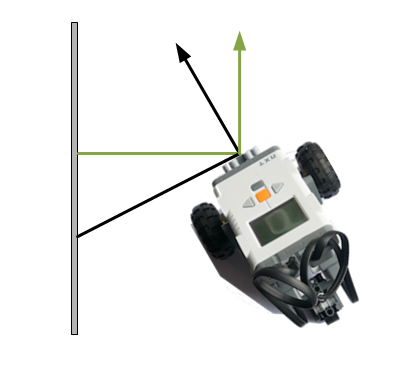
\includegraphics[width=80mm]{resources/muurvolger.png}
\end{figure}

Dankzij de richtbare sonar, kan de robot zowel de afstand tot de te volgen muur meten als voor zich controleren of er geen muur is, ten gevolge van een hoek in het parcours. De robot zal de sonar dus constant heen en weer laten bewegen om deze twee punten te controleren.

De implementatie van dit principe zal gebeuren aan de hand van een aparte thread die de constante beweging van de sonar regelt en meetwaarden ter beschikking stelt van de thread die het volgen van de muur implementeert. Initieel zal een zoekroutine voorzien worden om na te gaan of er een muur links of rechts dient gevolgd te worden.

Om deze richtbare sonar initieel recht vooruit te positioneren, voorzien we een automatische calibratie op basis van een v\'o\'or de robot opgesteld obstakel. De robot zal vervolgens de kortste afstand tot dit obstakel zoeken door de sonar te laten ronddraaien en metingen te doen.

\section{Testplan en resultaten}

In tegenstelling tot het rijden en de lichtsensor, verliepen de testen voor de sonarsensor anders: de sonarsensor meet constant dezelfde waarde in gelijke omstandigheden. Ook verschil in materiaal gaf zo goed als geen afwijkingen. We bekijken vervolgens metingen met de sonarsensor in een rechthoek tot een obstakel en het effect van een hoek op de meetresultaten. Tot slot bekijken we de invloed van rijden op het meten van afstanden.

\subsection{Afstand}

In een eerste test bepaalden we de afwijking op een afstandsmeting van 1 tot 60cm. Figuur \ref{chart:sonarDistance} geeft de absolute fout weer op verschillende gemeten afstanden.

\begin{figure}[htbp]
   \centering
   \caption{Test 1: Absolute afwijking van de sonarsensor tov de te meten afstand.}
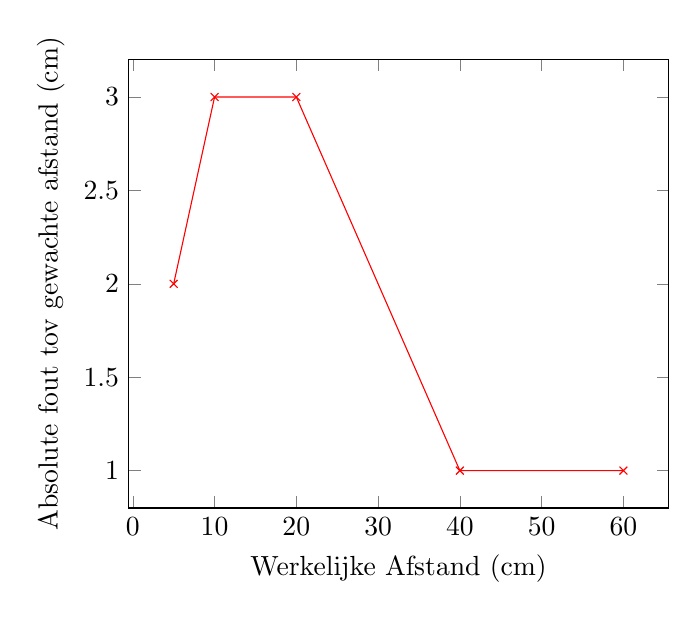
\begin{tikzpicture}
    \begin{axis}[
        xlabel=Werkelijke Afstand (cm),
        ylabel=Absolute fout tov gewachte afstand (cm)]
    \addplot[color=red,mark=x] coordinates {
	(5,2)
	(10,3)
	(20,3)
	(40,1)
	(60,1)
   };
    \end{axis}
\end{tikzpicture}
   \label{chart:sonarDistance}
\end{figure}

Hierbij valt onmiddellijk op dat de sonar beduidend correcter meet op grotere afstand en een grotere fout laat optekenen bij kleinere. Aangezien deze metingen nagenoeg constant waren, kunnen we deze meetgegevens gebruiken om een functie of vertaaltabel te maken tussen de metingen van de sonarsensor en de re\"ele afstand.

\subsection{Hoek}

Een robot zal niet steeds loodrecht staan t.o.v. een obstakel. Het principe van de sonarsensor berust op weerkaatsing van uitgezonden golven. Vanaf een hoek van 45 graden, zullen deze golven niet meer teruggekaatst worden. Elementaire testen toonden dit aan.

\subsection{Rijden}

De robot zal hoofdzakelijk metingen doen terwijl hij rijdt. Het is daarom interessant om te weten of dit een grote impact heeft. Een test werd gedaan waarbij de robot op een afstand van een obstakel werd geplaatst en naar het obstakel toe reed. Hierbij registreerde de robot informatie van de tachometer en van de sonarsensor. Op basis van deze gegevens kunnen we de metingen van de sonar afstemmen op de afstand berekend door de tachometer. We hebben verschillende metingen voor deze test gedaan en de meetresultaten waren telkens ongeveer identiek. Ze vertoonden ook een typisch patroon, zoals weergegeven in figuur \ref{chart:sonarDrive}.

\begin{figure}[htbp]
   \centering
   \caption{Test 3: Absolute fout van de sonarsensor bij rijdende meting.}
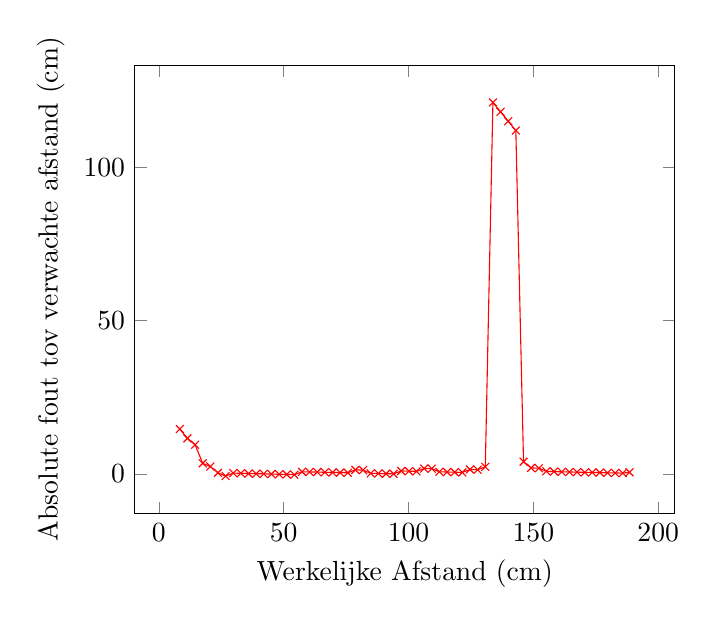
\begin{tikzpicture}
    \begin{axis}[
        xlabel=Werkelijke Afstand (cm),
        ylabel=Absolute fout tov verwachte afstand (cm),
       legend style={draw=none}]
    \addplot[color=red,mark=x,] coordinates {
(188.50,0.50)
(185.78,0.22)
(182.73,0.27)
(179.68,0.32)
(176.60,0.40)
(173.55,0.45)
(170.54,0.46)
(167.46,0.54)
(164.41,0.59)
(161.36,0.64)
(158.28,0.72)
(155.18,0.82)
(152.18,1.82)
(149.08,1.92)
(146.05,3.95)
(142.97,112.03)
(139.92,115.08)
(136.84,118.16)
(133.79,121.21)
(130.74,2.26)
(127.66,1.34)
(124.58,1.42)
(121.55,0.45)
(118.48,0.52)
(115.42,0.58)
(112.35,0.65)
(109.32,1.68)
(106.27,1.73)
(103.19,0.81)
(100.16,0.84)
(97.08,0.92)
(94.01,-0.01)
(90.98,0.02)
(87.90,0.10)
(84.85,0.15)
(81.80,1.20)
(78.72,1.28)
(75.67,0.33)
(72.61,0.39)
(69.56,0.44)
(66.51,0.49)
(63.43,0.57)
(60.40,0.60)
(57.35,0.65)
(54.30,-0.30)
(51.20,-0.20)
(48.15,-0.15)
(45.09,-0.09)
(42.02,-0.02)
(38.96,0.04)
(35.93,0.07)
(32.83,0.17)
(29.78,0.22)
(26.73,-0.73)
(23.68,0.32)
(20.62,2.38)
(17.57,3.43)
(14.52,9.48)
(11.44,11.56)
(8.41,14.59)
   };
    \end{axis}
\end{tikzpicture}
   \label{chart:sonarDrive}
\end{figure}

De robot vertrok op 180cm van het obstakel. Zoals we reeds opmerkten in de voorgaande testen, is de sonar relatief nauwkeurig op grotere afstanden. Vanaf 30cm vergroot de fout aanzienlijk.

Er is een piek die zich voordoet rond de 130 tot 140cm. Op deze afstand detecteert de sensor geen obstakels. We vermoeden dat er zich hier een eigenfrequentie optreedt en dat er golffronten samenvallen. Aangezien we voor de doelstellingen van de verschillende demo's geen informatie nodig hebben voor afstanden boven de 80cm, is dit fenomeen onbelangrijk voor ons. Deze observatie werd door andere groepen bevestigd.

De meetwaarden van deze test waren omvangrijk in aantal. Ze werden dan ook met behulp van de Bluetooth verbinding doorgestuurd naar de PC voor verdere verwerking in een spreadsheet.

\section{Resultaten van de demo en conclusies}

De robot was in staat om meerdere rondjes op het parcours te rijden. Het algoritme voorzag een robot die vooruitreed en veranderen slechts van richting op basis van een nieuwe volledige set van sonar-waarden. De tijd om een volledige ``sweep'' uit te voeren was echter soms te lang om tijdig van richting te veranderen om een obstakel te vermijden. Naar de finale demo toe willen we de verhouding tussen het rijden en het detecteren van obstakels met de sonar, verder verfijnen.

\chapter{Demo 2c: Barcode}

De doelstelling van de vierde demo is het detecteren van barcodes op een eenvoudig parcours. Op basis van de informatie die deze barcodes aanbieden moet de robot zijn weg vinden naar de volgende barcode en zo het parcours 1 keer afleggen.

\section{Fysiek ontwerp}

Voor het lezen van barcodes gebruiken we de grijswaardesensor. Deze is reeds op de robot gemonteerd, zoals besproken in sectie \ref{section:lichtsensor}. Eveneens de basissoftware om grijswaarden te registeren wordt opnieuw gebruikt.

\section{De software}

Het algoritme dat op basis van de gemeten grijswaarden barcodes doorloopt een oneindige lus, waarin steeds een genormaliseerde waarde van de grijdwaardesensor gelezen wordt. Op basis van de calibratiewaarden wordt deze waarde omgezet in een kleur: bruin, wit of zwart.

Algemeen kent het algoritme twee grote statussen:

\begin{enumerate}
\item Gewoon rijden, op zoek naar een barcode.
\item Een gevonden barcode bepalen.
\end{enumerate}

Bij het zoeken naar een barcode worden bruine metingen genegeerd. Niet-bruine waarden brengt het algoritme in een status waarbij de gevonden barcode bepaald wordt. In die status worden alle niet-bruine waarden bewaard tot er opnieuw 5 bruinwaarden opgemeten zijn. Indien er minstens 3 niet-bruine waarden opgemeten zijn, wordt een barcode bepaald.

Hiervoor worden de opgemeten waardes in 7 gelijke groepen verdeeld. Voor elk van deze groepen wordt het gemiddelde bepaald en vertaald naar wit of zwart. Deze 7 wit/zwart waarden kunnen vertaald worden naar een reeks van 1-en en 0-en, welke ge\"interpreteerd worden als een getal.

Tot slot wordt aan de hand van een tabel de effectief gedetecteerde waarde omgezet naar een gecorrigeerde waarde volgens de Hamming-code error-correctie.

\section{Testplan en resultaten}

De verschillende barcodes werden meermaals door de robot gedetecteerd, zowel recht-rijdend als onder verschillende hoeken. Alle testen resulteerden in een correct gelezen barcode.

\section{Resultaten van de demo en conclusies}

De robot detecteerde de barcodes correct, behalve de barcodes die zich op een helling bevonden. Om dit probleem op te lossen moeten we het fysieke ontwerp van de robot verder verfijnen, zodat de hoek van de helling geen negatieve impact heeft op de positie van de grijswaardesensor.

\chapter{Finale demonstratie}

Tijdens de finale demonstratie moet de robot autonoom een onbekend parcours rijden. Hierbij kan gebruik gemaakt worden van alle sensoren. Op het parcours kunnen panelen voorkomen waar maximaal \'e\'en sensor-waarneembare eigenschap weggenomen wordt.

\section{Fysiek ontwerp}

Het fysieke ontwerp van de robot is ongewijzigd gebleven sinds de vorige demo. We hadden tijdens die iteratie reeds de geplande aanpassingen gedaan. Een poging om een betere bevestiging van de lichtsensor te bekomen op basis van een parallellogram leverde geen noemenswaardige verbeteringen op. Met het oog op het rijden van een parcours beschouwen we het falen om een barcode te lezen als een eigenschap waar de robot bestand moet tegen zijn.

\section{De software}

Na de tussentijdse demo's zijn we voor het rijden van het parcours overgeschakeld op onze langere termijn strategie. Hiervoor werd een simulatieomgeving ontworpen om onafhankelijk van de fysieke robot te kunnen testen en experimenteren. We belichten de simulator kort, vooraleer we het eigenlijke huidige algoritme bespreken. Daarna bekijken we tevens kort het nieuwe logging framework en de nieuwe web-interface.

\subsection{Simulator}

Het ontwikkelen van software voor een door Lejos aangedreven Mindstorms robot, of eender welk ander ``embedded'' systeem, wordt typisch bemoeilijkt door de zeer beperkte toegankelijkheid van het systeem. Deze ontoegankelijkheid vertoont zich op verschillende vlakken: op fysiek vlak dient er steeds een nieuwe versie van de software overgebracht worden, moet de robot op een parcours geplaatst worden (dat eerst nog gebouwd moet worden), enz. Op vlak van software ontwikkeling is men niet in staat om normale ontwikkel-omgevingen te gebruiken en kan nauwelijks of met grote omwegen ``gedebugged'' worden.

We hebben daarom gekozen om een simulatieomgeving te cre\"eren waar we zelf alle controle over hebben en die de bovengenoemde problemen grotendeels oplost. Figuur \ref{fig:simulator} toont de simulator in actie.

\begin{figure}[htbp]
   \centering
   \caption{Simulator in actie.}
   \label{fig:simulator}
   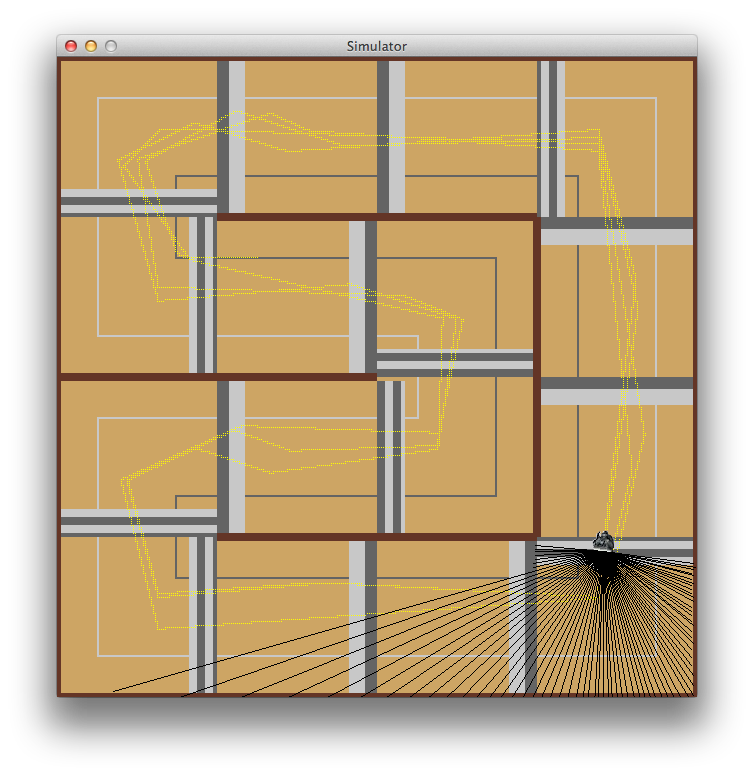
\includegraphics[width=150mm]{resources/simulator.png}
\end{figure}

De simulator stelt ons in staat om de exacte code die uiteindelijk op de robot zal gebruikt worden uit te voeren. Hierbij zal de simulatieomgeving de invoer voor de sensoren berekenen op basis van een voor-gedefinieerd parcours. De acties van de robot, uitgedrukt in veranderingen van de motoren, worden ook door de simulatieomgeving opgepikt en vervolgens omgezet in realistische verplaatsingen op het parcours.

\subsection{Model en Navigator}

In de event loop op de robot worden de verschillende sensor-waarden uitgelezen en in het \texttt{Model} gestopt. Vervolgens verwerken \texttt{ModelProcessoren} deze nieuwe waarden en voegen geaggregeerde informatie toe aan het model. Zo wordt informatie van de lichtsensor bijgehouden in een histogram, waarna barcodes of lijnen gedetecteerd kunnen worden.

Op basis van deze uitgebreide informatie over zijn wereld, zal vervolgens de \texttt{Navigator} bepalen welke actie er ondernomen dient te worden. Hierbij worden twee stappen doorlopen:

\begin{enumerate}
\item detecteren van events uit de wereld
\item uitvoeren van acties die zich op de \texttt{ActionQueue} bevinden.
\end{enumerate}

Tijdens het detecteren van de events uit de wereld, bekijkt de Navigator de volgende mogelijke gebeurtenissen in volgorde:

\begin{enumerate}
\item nabijheid van obstakels
\item detectie van barcodes
\item detectie van lijnen
\item botsing situaties
\end{enumerate}

Indien \'e\'en van deze gebeurtenissen voorvalt, zal de Navigator de nodige acties op de \texttt{ActionQueue} plaatsen. Dit is een queue van acties die ondernomen moeten worden. Zo zal bvb. bij een botsing er eerst achteruit gereden worden en vervolgens gedraaid worden.

De volgende acties staan ter beschikking van de Navigator:

\begin{itemize}
\item MoveAction
\item TurnAction
\item StopAction
\item DriveForwardAction
\item MoveOffLineAction // de robot draait tot zijn lichtsensor terug aan de andere kant van de lijn is
\end{itemize}

Elk van deze acties kan tot slot in een niet-onderbreekbare staat gebracht worden, waardoor er geen nieuwe events kunnen gedetecteerd worden.

Indien de robot geen acties meer in zijn queue heeft, gaat hij 'gap detection' gebruiken om zijn richting te bepalen. Als de robot met zijn sonar waarneemt dat hij in alle richtingen zal botsen, behalve in 1 duidelijk begrensde richting (the gap), dan zal de robot zich richting naar die gap.

Als er uit alle voorgaande condities niets van besloten worden, rijdt de robot gewoon vooruit.

\subsection{Logging en Web-interface}

Naast de overschakeling naar de model-gedreven navigator, is ook de manier van het verwerken van feedback van de robot gewijzigd. De robot zendt nu de informatie uit het model en de navigator door naar de PC. Deze gegevens worden nu niet langer rechtstreeks getoond in een grafische gebruikersinterface, maar worden via het log4j logging framework zo snel mogelijk in een relationele databank opgeslagen. Aan de hand van een REST-ful web-service, aangeboden van op een JBoss applicatie server, wordt nu de informatie weergegeven op een HTML/CSS/Javascript-gebaseerde interface. Figuur \ref{fig:webclient} toont de nieuwe web interface.

\begin{figure}[htbp]
   \centering
   \caption{De nieuwe webclient.}
   \label{fig:webclient}
   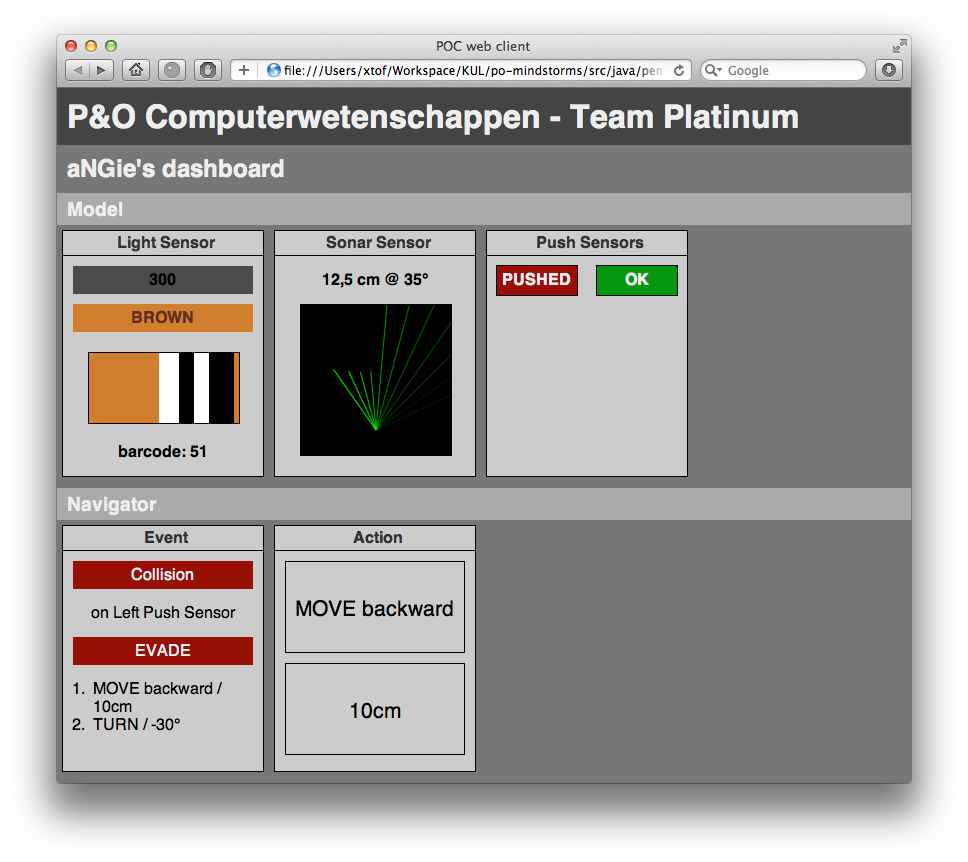
\includegraphics[width=150mm]{resources/webclient.png}
\end{figure}

De web interface tracht een getrouw beeld te geven van de informatie die zich op een bepaald moment in de software op de robot bevindt. Zo wordt het model en de navigator onafhankelijk voorgesteld. Binnen het model worden de verschillende sensoren weergegeven, met hun gemeten waarden, alsook de interpretatie ervan. De histogrammen van de licht- en sonar-sensoren, die in het model van de robot worden opgebouwd worden ook weergegeven in de interface.

\section{Resultaten van de demo en conclusies}

Dit deel wordt later toegevoegd.

\chapter{Het process}

Dit deel wordt later toegevoegd.

\chapter{Werkverdeling}

\begin{longtable}{l l}
\caption{Focus van elk team lid} \\ [0.5ex]
%This is the header for the first page of the table...
\hline\hline
Teamlid & Focus \\ [0.5ex]
\hline 
\endfirsthead
%This is the header for the remaining page(s) of the table...
\multicolumn{2}{c}{{\tablename} \thetable{} -- Vervolg} \\[0.5ex]
\hline \hline
Teamlid & Focus \\ [0.5ex]
\hline 
\endhead
Michiel 		& 	(Coordinator) Bluetooth communicatie, calibratie, finale navigator. \\
Florian 		&	RobotAPI, lijnvolger, opvolgen unit testen, finale navigator. \\
Ruben 		&	RobotAPI, veelhoek algoritme, muurvolger, sonar-navigator.\\
Thomas 		&	RobotAPI, lichtsensor, barcode-lezer, fat client. \\
Daniel 		&	Testen, barcode-lezer, fat client. \\
Christophe 	&	(Secretaris) Verslag, simulator, model \& navigator, web-client. \\
\hline
\label{tab:focus}
\end{longtable}

\begin{longtable}{l r r r r r r}
\caption{Tijdsbesteding per team lid per week} \\
%This is the header for the first page of the table...
\hline\hline
 & Michiel & Florian & Ruben & Thomas & Daniel & Christophe \\
\hline 
\endfirsthead
%This is the header for the remaining page(s) of the table...
\multicolumn{4}{c}{{\tablename} \thetable{} -- Vervolg} \\
\hline \hline
 & Michiel & Florian & Ruben & Thomas & Daniel & Christophe \\
\hline 
\endhead
totaal    & 121 & 90 & 91 & 76 & 78 & 128 \\
\hline
week 1 & 10 & 10 & 10 & 10 & 10 & 15 \\
week 2 & 9 & 7 & 8 & 7 & 9 & 16 \\
week 3 & 8 & 8 & 8 & 8 & 5 & 12 \\
week 4 & 9 & 7 & 5 & 8 & 5 & 17 \\
week 5 & 42 & 15 & 18 & 6 & 15 & 34 \\
week 6  & 15 & 11 & 12 & 18 & 15 & 5 \\
week 7 & 5 & 11 & 10 & 9 & 9 & 9 \\
week 8 & 10 & 9 & 12 & 5 & 5 & 9 \\
week 9 & 13 & 12 & 8 & 5 & 5 & 11\\
week 10 \\
week 11 \\
\hline
\label{tab:tijdsregistratie}
\end{longtable}

\chapter{Analyse}

Dit deel wordt later toegevoegd.

\appendix

\chapter{Software}
\label{appendix:software}

\section{Bluetooth}
\label{appendix:bluetooth}

Dit deel wordt later toegevoegd.

\section{Klasse Diagrammen}
\label{appendix:classDiagrams}

Dit deel wordt later toegevoegd.

\section{Overzicht Methodes}

Dit deel wordt later toegevoegd.

\section{Functionaliteit}

Dit deel wordt later toegevoegd.

\section{Simulator}

Dit deel wordt later toegevoegd.

\chapter{User Interface}
\label{appendix:ui}

Dit deel wordt later toegevoegd.

\section{Design}

Dit deel wordt later toegevoegd.

\section{Functionaliteit}

Dit deel wordt later toegevoegd.

\chapter{Work Breakdown Structure}
\label{appendix:wbs}

\begin{longtable}{r l l c}
\caption{Work Breakdown Structure} \\ [0.5ex]
%This is the header for the first page of the table...
\hline\hline
\# & Omschrijving & Verantwoordelijke & Milestone \\ [0.5ex]
\hline 
\endfirsthead
%This is the header for the remaining page(s) of the table...
\multicolumn{4}{c}{{\tablename} \thetable{} -- Vervolg} \\[0.5ex]
\hline \hline
\# & Omschrijving & Verantwoordelijke & Milestone \\ [0.5ex]
\hline 
\endhead
1	& bepalen optimaal algoritme/verplaatsing	& 					& Demo 1\\
1,1	& codering robot API met tijd/snelheid		& Michiel				& \\
1.2	& codering robot API met omwentelingen		& Ruben				& \\
1.3	& codering tests : tijd/snelheid				& Michiel, Florian 		& \\
1.4	& codering tests : omwentelingen			& Michiel				& \\
1.5	& uitvoeren alle tests, metingen,...			& Ruben, Daniel		& \\
2	& implementatie veelhoek oplossing		& Ruben				& Demo 1 \\
3	& ontwikkeling LCD menu				& Thomas				& \\
4	& verslag voorbereiden					& 					& \\
4.1	& voor demo 1							& Christophe			& Demo 1 \\
4.2	& voor demo 2							& Christophe			& Demo 2 \\
4.3	& voor finale demo						& Christophe			& Finale \\
5	& ontwikkeling communicatie component		&					& \\		
5.1	& ontwikkeling communicatie thread			&					& \\
5.1.1	& ontwikkeling log kanaal					& Ruben				& Demo 2 \\
5.1.2	& ontwikkeling commando kanaal			& Michiel				& \\
5.2	& ontwikkeling robot agent				&					& \\		
5.2.1	& ontwikkeling log kanaal					& Ruben				& Demo 2 \\
5.2.2	& ontwikkeling commando kanaal			& Michiel				& \\
6	& ontwikkeling model component			& Christophe			& Final \\
7	& ontwikkeling navigator					&					& \\
7.1	& ontwikkeling abstracte navigator			& Christophe			& \\
7.2	& design concrete navigator				&					& \\
7.3	& implementatie concrete navigator			&					& \\
7.4	& testen concrete navigator				&					& \\
8	& ontwikkeling simulator					& Christophe			& \\
9	& ontwikkeling log server					& Michiel, Ruben		& Demo 2 \\
10	& opzetten syslog, file, tail -f mini-client		& Michiel, Ruben		& Demo 2 \\
11	& opzetten database server				& Christophe			& \\
12	& ontwikkeling Fat Client					&					& \\	
12.1	& weergave robot status uit database		& Michiel				& (Demo 2) \\
12.2	& implementatie commando�s				& Michiel				& \\
13	& ontwikkeling SOA						&					& \\
13.1	& opzetten REST service					& Christophe, Ruben 	& \\
13.2	& ontwikkeling web client					& Christophe, Ruben	& \\
14	& ontwikkeling Smart client				& Florian, Thomas		& \\
15	& ontwikkeling zelf-calibratie				& Ruben, Daniel		& \\
16	& controle, vervolledigen unit testen			& Florian				& \\
17	& demo 2 : lijnvolger						& 					& Demo 2 \\
17.1	& onderzoek lichtsensor					& Thomas				& \\
17.2	& implementatie lichtsensor				&					& \\	
17.3	& implementatie lijnvolger				& Thomas, Florian		& \\
18	& demo 2 : muurvolger					& 					& Demo 2 \\
18.1	& onderzoek sonarsensor					& Ruben				& \\
18.2	& implementatie sonarsensor				& Ruben				& \\
18.3	& implementatie muurvolger				&					& \\	
19	& demo 2 : barcode						& 					& Demo 2 \\
19.1	& onderzoek detectie barcodes			& Thomas, Daniel		& \\
19.2	& implementatie barcode					&					& \\	
19.3	& implementatie barcode lezer				&					& \\
\hline
\label{tab:wbs}
\end{longtable}

\chapter{Planning}
\label{appendix:planning}

\begin{figure}[htbp]
\centering
\begin{tikzpicture}
	\begin{ganttchart}[ 
	  y unit title=0.6cm,
	  y unit chart=0.5cm,
	  vgrid,
	  bar height=.5,
	  group right shift=0,
	  group top shift=.6,
	  group height=.3]{22}
\gantttitle{Oktober}{10} 	   	\gantttitle{November}{8} 	    \gantttitle{December}{4} \\
\gantttitlelist{3,10,17,24,31}{2}	\gantttitlelist{7,14,21,28}{2}  \gantttitlelist{5,12}{2} \\
\ganttgroup{1. Beweging}{1}{5} \\
\ganttbar{1.1. API Tijd}{2}{4} \\
\ganttbar{1.2. API Omw.}{2}{4} \\
\ganttbar{1.3. Tijd}{4}{5} \\
\ganttbar{1.4. Omw.}{4}{5} \\
\ganttbar{1.5. tests}{5}{5} \\
\ganttbar{2. Veelhoek}{3}{5} \\
\ganttbar{3. LCD}{2}{5} \\
\ganttmilestone{Demo 1}{5} \ganttnewline
\ganttgroup{4. Verslag}{1}{20} \\
\ganttbar{4.1. Demo 1}{2}{5} \\
\ganttbar{4.2. Demo 2}{8}{12} \\
\ganttbar{4.3. Finaal}{18}{20} \\
\ganttgroup{5. Comm.}{3}{20} \\
\ganttgroup{5.1. Robot}{3}{20} \\
\ganttbar{5.1.1. Log}{3}{11} \\
\ganttbar{5.1.2. Commando}{11}{20} \\
\ganttgroup{5.2. PC}{5}{20} \\
\ganttbar{5.2.1. Log}{5}{11} \\
\ganttbar{5.2.2. Commando}{11}{20} \\
\ganttbar{6. Model}{3}{18} \\
\end{ganttchart}
\end{tikzpicture}
\caption{Planning}
\label{fig:planning}
\end{figure}

\begin{figure}[htbp]
\centering
\begin{tikzpicture}
	\begin{ganttchart}[ y unit title=0.6cm, y unit chart=0.5cm,  vgrid,
	  bar height=.5,
	  group right shift=0,
	  group top shift=.6,
	  group height=.3]{22}
\gantttitle{Oktober}{10} 	   	\gantttitle{November}{8} 	    \gantttitle{December}{4} \\
\gantttitlelist{3,10,17,24,31}{2}	\gantttitlelist{7,14,21,28}{2}  \gantttitlelist{5,12}{2} \\
\ganttgroup{7. Navigator}{5}{18} \\
\ganttbar{7.1. Abstract}{5}{11} \\
\ganttbar{7.2. Design}{11}{18} \\
\ganttbar{7.3. Impl.}{13}{18} \\
\ganttbar{7.4. Tests}{15}{18} \\
\ganttbar{8. Simulator}{3}{13} \\
\ganttbar{9. Log server}{5}{11} \\
\ganttbar{10. Syslog}{7}{10} \\
\ganttbar{11. DB server}{7}{10} \\
\ganttgroup{12. Fat client}{9}{16} \\
\ganttbar{12.1. Status}{9}{14} \\
\ganttbar{12.2. Commando}{10}{16} \\
\ganttgroup{13. SOA}{9}{12} \\
\ganttbar{13.1. REST}{9}{11} \\
\ganttbar{13.2. web client}{10}{12} \\
\ganttbar{14. Smart client}{12}{18} \\
\ganttbar{15. Calibratie}{12}{18} \\
\ganttbar{16. Unit tests}{2}{18} \\
\ganttgroup{17. Lijnvolger}{5}{10} \\
\ganttbar{17.1. Onderzoek}{5}{8} \\
\ganttbar{17.2. Sensor}{7}{9} \\
\ganttbar{17.3. Impl.}{9}{10} \\
\ganttgroup{18. Muurvolger}{5}{10} \\
\ganttbar{18.1. Onderzoek}{5}{8} \\
\ganttbar{18.2. Sensor}{7}{9} \\
\ganttbar{18.3. Impl.}{9}{10} \\
\ganttgroup{19. Barcode}{5}{10} \\
\ganttbar{19.1. Onderzoek}{5}{8} \\
\ganttbar{19.2. Detectie}{7}{9} \\
\ganttbar{19.3. Impl.}{9}{10} \\
\ganttmilestone{Demo 2}{10} \ganttnewline
\ganttmilestone{Finale Demo}{18} \ganttnewline
\ganttbar{20. Finaal verslag}{19}{20} \\
\end{ganttchart}
\end{tikzpicture}
\caption{Planning (vervolg)}
\label{fig:planning2}
\end{figure}

\end{document}
